
\textbf{Hadron Calorimetry for SiD, [PI: White]} \
UTA has for several years worked on the development of hadron calorimetry for a future lepton collider.
Our graduate and undergraduate students have benefitted significantly from participation in this work,
and have made valuable contributions.
Future experiments make severe demands on achieving excellent the jet energy resolution.
Much of the new physics program for the ILC requires high-precision measurements of jet
energies and jet-jet invariant masses.  Studies have shown that there is a basic requirement of at least $30\%/\sqrt{E}$,
at 100GeV or 3-4\% in general for jet energy resolution. 
This need arises from the requirement for precision Higgs studies, and precision measurements
of the masses and other properties of new particles that may be discovered in the next few years at the LHC.
A prime physics example of the need for this precision is the reconstruction and 
separation of hadronic decay modes of W and Z bosons, on an event-by-event basis. 
Hence there has existed a need for the development of a new type of hadron calorimetry.

The hadron calorimeter is an essential component of the Particle Flow Algorithm (PFA) approach to achieving the required
jet energy resolution. The PFA approach has been developed and extensively used in physics studies by both the 
main ILC detector groups, SiD and ILD. It has also been used in LHC jet reconstruction. Most of the calorimeter 
development work to provide technical solutions to implementing PFA-orineted systems has been carried out by the 
CALICE Collaboartion (Ref.). White and Felix Sefkow (DESY) (joined by K. Kawagoe, R. Pöschl, and J. Repond) were 
asked to be the authors/main editors of a Reviews of Modern Physics paper on "Experimental tests of particle flow calorimetry".
This paper was published \cite{RMPCALICE} in early 2016 and represents a atatement and synthesis of developments of PFA calorimetry.
As reflected by this paper, there has emerged a choice of technologies in which to implement the hadron calorimeter for SiD.
The technology must support individual charged particle tracking through the calorimeter, allow detailed imaging of energy 
depositions for track-shower association and separation of closeby showers, while providing good energy resolution for the
direct measurement of the energies of neutral particles.
White proposed \cite{GEMDHCAL} a digital hadron calorimeter implementation using Gas Electron Multiplier (GEM) technology ~\cite{Sauli}.
GEM offers a robust solution with sufficient amplification in a double-foil configuration, and a thin active layer. 
This last requirement is important since a typical lepton collider hadron calorimeter would have about forty layers, with the 
entire system contained inside superconducting coil -- the cost of which must be limited.

Figure~\ref{fig:GEM_DHCAL_Schematic} shows the basic GEM-DHCAL idea introduced by White. The concept of embedding the front-end 
electronics as part of the active layer has been realized through the development of the KPiX 1024-channel chip by SLAC (with a series of 
earlier versions also having been tested at UTA). KPiX is specifically designed for the time structure of the ILC beam, and requires a 
synchronous environment to operate at full efficiency. To implement a full digital hadron calorimeter system would clearly require 
large area chambers. UTA has developed a series of prototype GEM-DHCAL chambers (see Figure~\ref{fig:GEM_DHCAL_2} ) with fine ($1cm \times 1cm$) cells. 
A key characteristic of an active layer suitable for use in a digital hadron calorimeter is a low hit multiplicity per track per layer 
while maintaining a high hit efficiency. Figure~\ref{fig:Eff_mult} shows that our GEM chamber(s) indeed have this desired
performance characteristic. The GEM-DHCAL development work has given us very valuable experience with respect to the implementation
of the hadron calorimeter for SiD.

\begin{figure}[htb]
\centering
%
\subfigure[]{%
      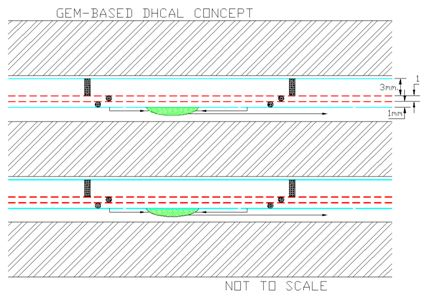
\includegraphics[scale=0.4]{images/GEM_DHCAL_Schematic.jpg}
      \label{fig:GEM_DHCAL_Schematic}
           }
%
\quad
\subfigure[]{%
      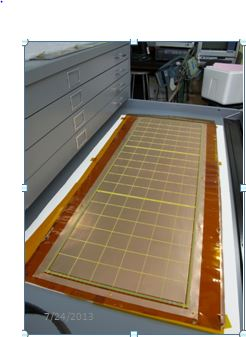
\includegraphics[scale=0.4]{images/GEM_DHCAL_2.jpg}
      \label{fig:GEM_DHCAL_2}
           }
%
%
\quad
\subfigure[]{%
       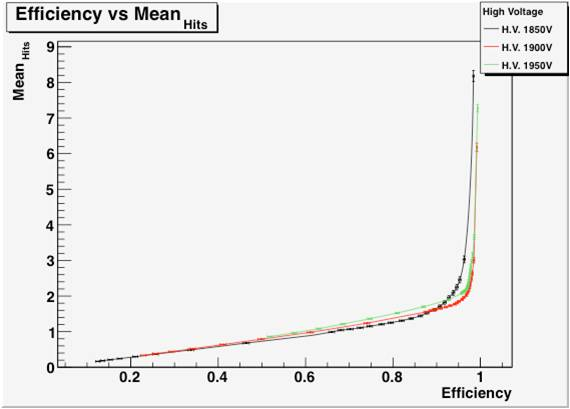
\includegraphics[scale=0.4]{images/Eff_Mult_GEM_DHCAL.jpg}
       \label{fig:Eff_mult}
           }

\caption{(a) GEM Digital Hadron Calorimeter Schematic. (b) large chamber under construction. 
(c) Multiplicity vs. hit efficiency.}
\end{figure}

The recently adopted, and current, baseline technology for the SiD hadron calorimeter, for detector simulation and physics studies, is small 
scintillator tiles with SiPM readout, and steel absorber plates. This approach has been the subject of considerable work by CALICE. 

UTA plans to take a leading role within SiD in the development, design, prototyping, and construction of the SiD hadron calorimeter system 
based on the scintillator/SiPM/steel technology. As a first step, UTA has undertaken the implementation of this technology in the DD4HEP \cite{DD4HEP} 
framework for the SiD simulation. White has been working with two undergraduate students to specify the details of the hadron calorimeter 
simulation. Figure~\ref{fig:AHCAL_Schematic} shows the CALICE design for an active layer, and the details of its realization for the SiD simulation.
CALICE studies have shown that $3cm \times 3cm$ cells yield the required jet energy resolution, and we have used this cell size for SiD.
Figure~\ref{fig:SiD_Barrel_single} shows the first result for the barrel simulation with a single incident charged particle. Once the full hadron calorimeter 
simulation is complete, we will make extensive comparisons between our simulations and the results of the CALICE beam tests for a variety of incident
particles. 
SiD has chosen a 12-fold design for the hadron calorimeter (see Figure~\ref{fig:SiD_AHCAL_12_sided}). taking the CALICE active layer design as input, we will 
develop a 40-layer module design. This will require the construction and testing of a representative size prototype of an active layer,
specification of layer assembly techniques (possibly automated), and mechanical module prototypes.

\begin{figure}[htb]
\centering
%
\subfigure[]{%
      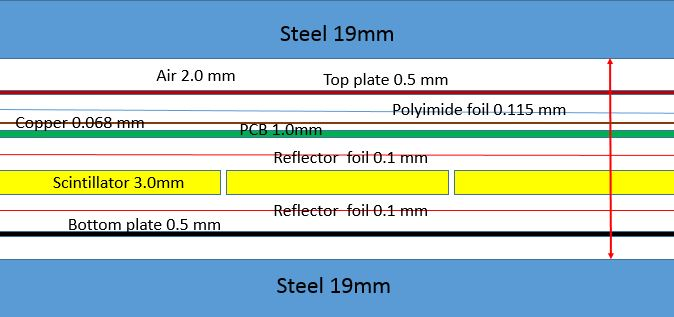
\includegraphics[scale=0.3]{images/AHCAL_Schematic.JPG}
      \label{fig:AHCAL_Schematic}
           }
%
\quad
\subfigure[]{%
      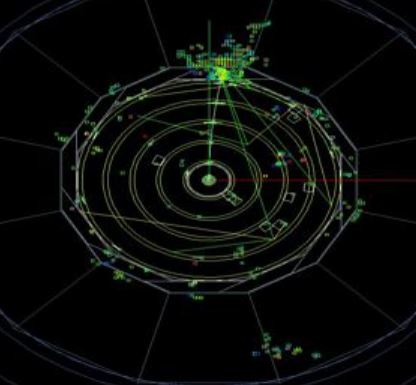
\includegraphics[scale=0.3]{images/SiD_Barrel_single.JPG}
      \label{fig:SiD_Barrel_single}
           }
%
%
\quad
\subfigure[]{%
       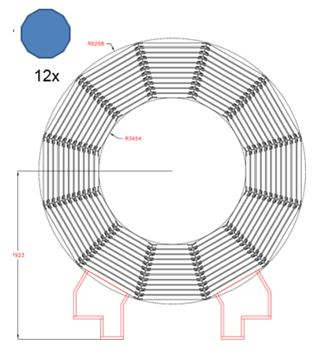
\includegraphics[scale=0.5]{images/SiD_AHCAL_12_sided.JPG}
       \label{fig:SiD_AHCAL_12_sided}
           }

\caption{(a) SiD AHCAL Barrel layer schematic. (b) SiD AHCAL simulation - single pion. 
(c) SiD AHCAL Barrel 12-sided structure.}
\end{figure}

All this activity will be a precursor to the SiD Technical Design Report, the timescale for which depends on the overall progress on the
ILC project. We anticipate 2-3 years to complete the TDR, once resources are available.

\textbf{SiD Timetable of Activities}
A decision on the ILC Project is expected in 2018. This timetable reflects this anticipated schedule.
The activities below reflect White's role as SiD Spokesperson and the planned work at UTA on the SiD hadron calorimeter.

\textbf{2017}
\begin{itemize}[noitemsep,nolistsep]
\item{Guide and pursue the optimization studies for all SiD subsystems}
\item{Initiate and guide further physics studies in response to new LHC results}
\item{Expand the SiD Consortium, particularly in Europe and Asia}
\item{Work with the U.S.- Japan Caucus and the ALCC to prepare the case for U.S. support of the ILC}
\item{Represent SiD at national and international Linear Collider conferences}
\item{Complete the full simulation of the SiD baseline hadron calorimeter, and verify performance vs. CALICE results}
\item{Develop initial hadron calorimeter barrel and endcap module concepts}
\end{itemize}

\textbf{2018}
\begin{itemize}[noitemsep,nolistsep]
\item{Continue the first five tasks from 2017}
\item{Work with Japanese colleagues to provide input from SiD to inform the anticipated ILC Project decision by MEXT}
\item{Begin the framework for the SiD Technical Design Report}
\item{Develop production and assembly procedures for SiD hadron calorimeter actve layers, and module integration}
\end{itemize}


\textbf{2019}
Subject to the ILC Project proceeding:
\begin{itemize}[noitemsep,nolistsep]
\item{Continue the general tasks from 2017/18}
\item{Prepare the SiD Experiment initial submission in response to anticipated call for expressions of interest/proposals}
\item{Establish initial areas of responsibilities for SiD member institutes in the transition from the SiD Consortium to the SiD Collaboration}
\item{Begin full engineering design and prototyping for SiD hadron calorimeter modules}
\end{itemize}


